\section{Results}
The results presented for each scenario include the energy produced, reactor 
deployment schedule, natural
uranium mass, \gls{HALEU} mass, and \gls{SWU} capacity as a function of time. 

\subsection{Scenario 1}
The amount of energy supplied by the \glspl{LWR} and the number of \glspl{LWR}
deployed as a function of time is shown in Figure \ref{fig:energy_rx_1}. 
\glspl{LWR} are first deployed in August of 1967, and the last 
\gls{LWR} is decommissioned in June of 2016. The maximum number of 
\glspl{LWR} deployed at one time is 109. The enery produced by the 
\glspl{LWR} follows with the number of reactors deployed. The maximum energy 
produced by the \glspl{LWR} is 102.46 GWe-y, and they produce 91.82 GWe-y 
in 2025.

\begin{figure}
    \centering 
    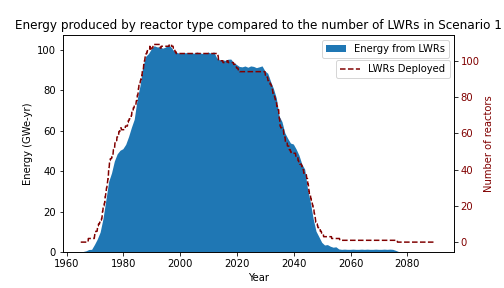
\includegraphics[scale=0.5]{figures/energy_scenario1.png}
    \caption{Energy supplied by \glspl{LWR} compared to the number of 
    \glspl{LWR} deployed in Scenario 1.}
    \label{fig:energy_rx_1}
\end{figure}

The next result is the amount of uranium sent to the \glspl{LWR} to fuel 
them, as shown in Figure \ref{fig:fuel_1}.

\begin{figure}
    \centering 
    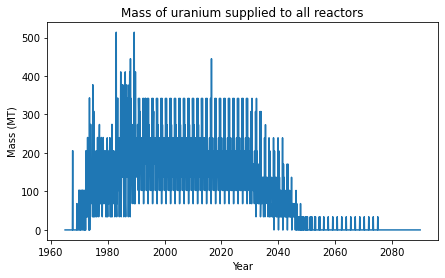
\includegraphics[scale=0.5]{figures/fuelsupply_scenarios_1.png}
    \caption{Mass of uranium sent to reactors in Scenario 1.}
    \label{fig:fuel_1}
\end{figure}

Finally, the \gls{SWU} capacity to produce fuel for the scenario, shown in 
Figure \ref{fig:swu_1}. 

\begin{figure}
    \centering
    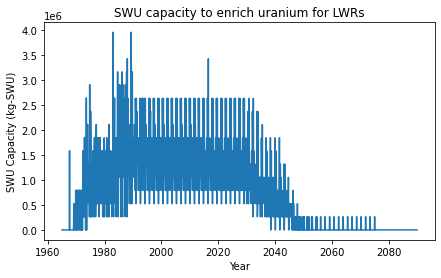
\includegraphics[scale=0.5]{figures/totalswu_scenarios_1.png}
    \caption{Total \gls{SWU} capacity required to produce fuel sent to the 
    reactors at each time step in Scenario 1.}
    \label{fig:swu_1}
\end{figure}


Each of the metrics from this scenario, the \gls{LWR} deployment schedule, 
energy supplied by them, uranium mass used to fuel the reactors, and the 
\gls{SWU} capacity needed to produce their fuel are the same for each of 
the other scenarios. 

\subsection{Scenario 2}
The energy produced by each type of reactor, the transition energy demand, 
and the deployment schedule of the \glspl{MMR} for Scenario 2 are shown in 
Figure \ref{fig:energy_rx_2}. Once the transition begins in 2025, there are 
clearly some time periods in which the energy demand of the scenario is 
not met. The first of these is between 2030-2050, with a maximum defecit 
of . Other periods in which the energy demand is not met correspond to 
the decommissioning of \glspl{MMR} at the end of their lifetime and the 
deployment of new reactors. 

The first \glspl{MMR} are deployed starting in October 2031, and the 
maximum number of \glspl{MMR} deployed at one time in this scenario is 
9,182. 

\begin{figure}
    \centering 
    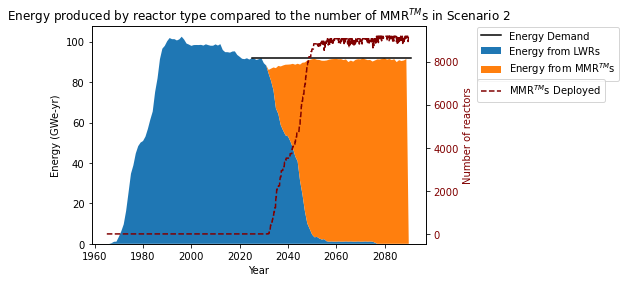
\includegraphics[scale=0.5]{figures/energy_scenario2.png}
    \caption{Energy supplied by each type of reactor compared to the number of 
    \glspl{MMR} deployed in Scenario 2.}
    \label{fig:energy_rx_2}
\end{figure}



\begin{figure}
    \centering
    \begin{subfigure}{0.4\textwidth}
        \centering
        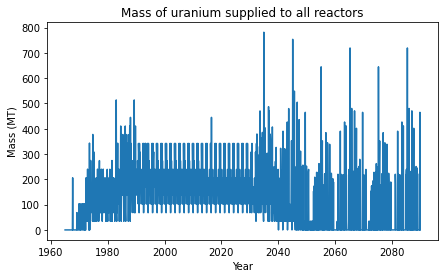
\includegraphics[scale=0.3]{figures/fuelsupply_scenarios_2.png}
        \caption{Total mass of uranium sent to all reactors at each time step.}
        \label{fig:totalfuel_2}
    \end{subfigure}
    \begin{subfigure}{0.4\textwidth}
        \centering
        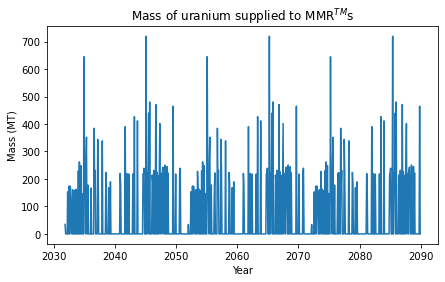
\includegraphics[scale=0.3]{figures/advancedRX_fuelsupply_scenarios_2.png}
        \caption{Total mass of uranium sent to \glspl{MMR} at each time step.}
        \label{fig:haleu_2}
    \end{subfigure}
    \caption{Uranium mass sent to reactors in Scenario 2.}
    \label{fig:fuel_2}
\end{figure}


\begin{figure}
    \centering
    \begin{subfigure}{0.4\textwidth}
        \centering
        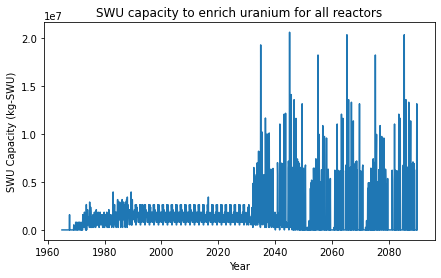
\includegraphics[scale=0.3]{figures/totalswu_scenarios_2.png}
        \caption{Total \gls{SWU} required to enrich uranium sent to all reactors at each time step.}
        \label{fig:totalswu_2}
    \end{subfigure}
    \begin{subfigure}{0.4\textwidth}
        \centering
        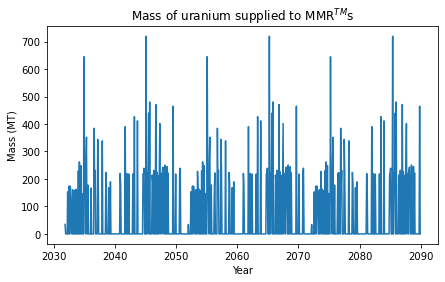
\includegraphics[scale=0.3]{figures/advancedRX_fuelsupply_scenarios_2.png}
        \caption{\gls{SWU} required to enrich uranium sent to \glspl{MMR} at each time step.}
        \label{fig:haleuswu_2}
    \end{subfigure}
    \caption{\gls{SWU} required to enrich natural uranium in Scenario 2.}
    \label{fig:swu_2}
\end{figure}

\subsection{Scenario 3}

\begin{figure}
    \centering 
    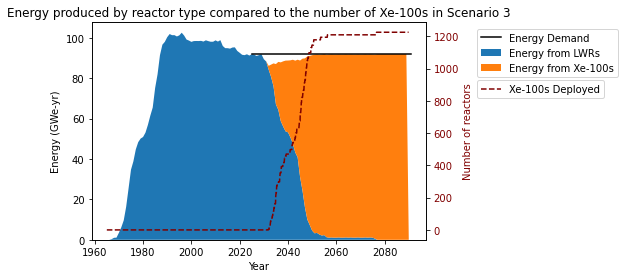
\includegraphics[scale=0.5]{figures/energy_scenario3.png}
    \caption{Energy supplied by each type of reactor compared to the number of 
    Xe-100s deployed in Scenario 3.}
    \label{fig:energy_rx_3}
\end{figure}

\begin{figure}
    \centering
    \begin{subfigure}{0.4\textwidth}
        \centering
        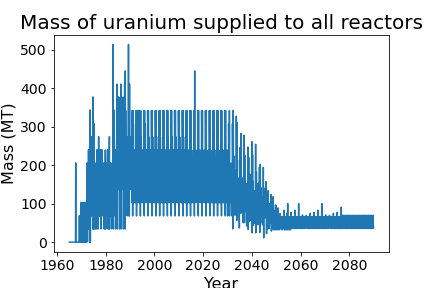
\includegraphics[scale=0.3]{figures/fuelsupply_scenarios_3.png}
        \caption{Total mass of uranium sent to all reactors at each time step.}
        \label{fig:totalfuel_3}
    \end{subfigure}
    \begin{subfigure}{0.4\textwidth}
        \centering
        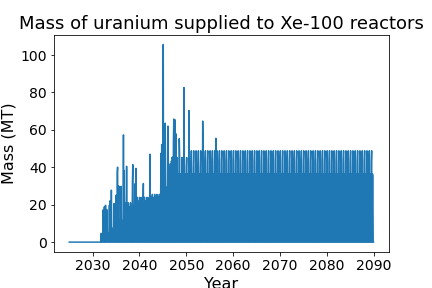
\includegraphics[scale=0.3]{figures/advancedRX_fuelsupply_scenarios_3.png}
        \caption{Total mass of uranium sent to Xe-100s at each time step.}
        \label{fig:haleu_3}
    \end{subfigure}
    \caption{Uranium mass sent to reactors in Scenario 3.}
    \label{fig:fuel_3}
\end{figure}


\begin{figure}
    \centering
    \begin{subfigure}{0.4\textwidth}
        \centering
        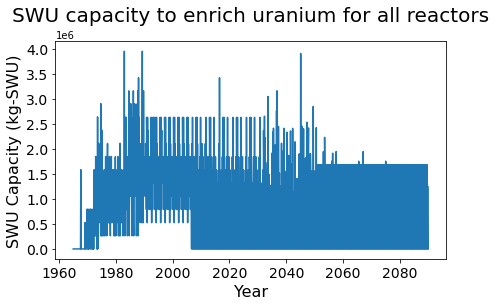
\includegraphics[scale=0.3]{figures/totalswu_scenarios_3.png}
        \caption{Total \gls{SWU} required to enrich uranium sent to all reactors at each time step.}
        \label{fig:totalswu_3}
    \end{subfigure}
    \begin{subfigure}{0.4\textwidth}
        \centering
        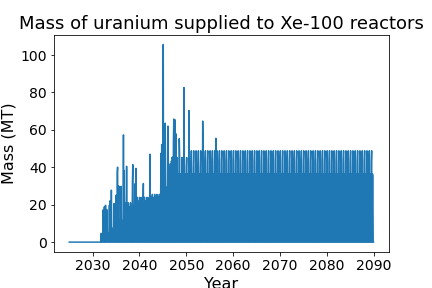
\includegraphics[scale=0.3]{figures/advancedRX_fuelsupply_scenarios_3.png}
        \caption{\gls{SWU} required to enrich uranium sent to Xe-100s at each time step.}
        \label{fig:haleuswu_3}
    \end{subfigure}
    \caption{\gls{SWU} required to enrich natural uranium in Scenario 3.}
    \label{fig:swu_3}
\end{figure}

\subsection{Scenario 4}

\begin{figure}
    \centering 
    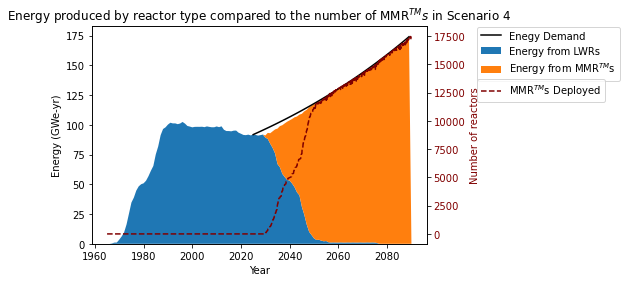
\includegraphics[scale=0.5]{figures/energy_scenario4.png}
    \caption{Energy supplied by each type of reactor compared to the number of 
    \glspl{MMR} deployed in Scenario 4.}
    \label{fig:energy_rx_4}
\end{figure}


\begin{figure}
    \centering
    \begin{subfigure}{0.4\textwidth}
        \centering
        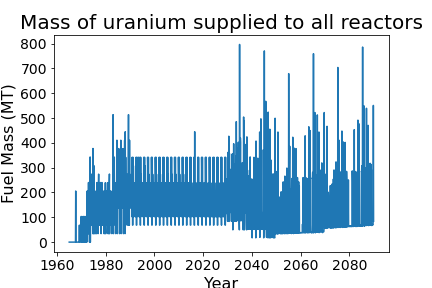
\includegraphics[scale=0.3]{figures/fuelsupply_scenarios_4.png}
        \caption{Total mass of uranium sent to all reactors at each time step.}
        \label{fig:totalfuel_4}
    \end{subfigure}
    \begin{subfigure}{0.4\textwidth}
        \centering
        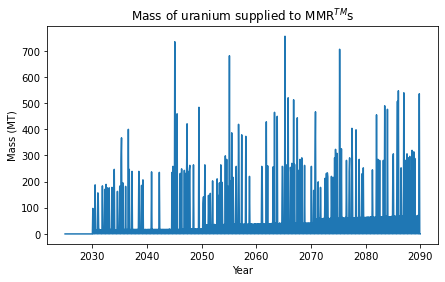
\includegraphics[scale=0.3]{figures/advancedRX_fuelsupply_scenarios_4.png}
        \caption{Total mass of uranium sent to \glspl{MMR} at each time step.}
        \label{fig:haleu_4}
    \end{subfigure}
    \caption{Uranium mass sent to reactors in Scenario 4.}
    \label{fig:fuel_4}
\end{figure}


\begin{figure}
    \centering
    \begin{subfigure}{0.4\textwidth}
        \centering
        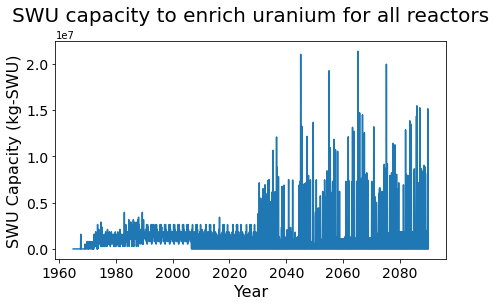
\includegraphics[scale=0.3]{figures/totalswu_scenarios_4.png}
        \caption{Total \gls{SWU} required to enrich uranium sent to all reactors at each time step.}
        \label{fig:totalswu_4}
    \end{subfigure}
    \begin{subfigure}{0.4\textwidth}
        \centering
        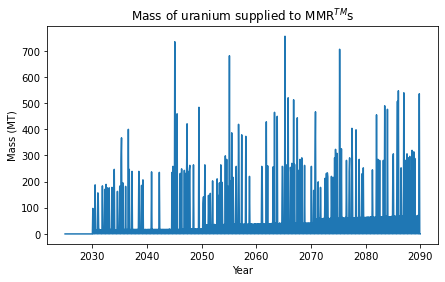
\includegraphics[scale=0.3]{figures/advancedRX_fuelsupply_scenarios_4.png}
        \caption{\gls{SWU} required to enrich uranium sent to \glspl{MMR} at each time step.}
        \label{fig:haleuswu_4}
    \end{subfigure}
    \caption{\gls{SWU} required to enrich natural uranium in Scenario 4.}
    \label{fig:swu_4}
\end{figure}
\subsection{Scenario 5}

\begin{figure}
    \centering 
    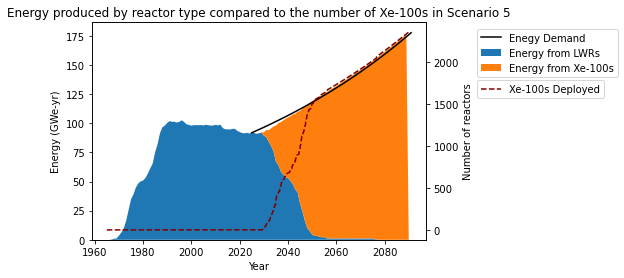
\includegraphics[scale=0.5]{figures/energy_scenario5.png}
    \caption{Energy supplied by each type of reactor compared to the number of 
    Xe-100s deployed in Scenario 5.}
    \label{fig:energy_rx_5}
\end{figure}

\begin{figure}
    \centering
    \begin{subfigure}{0.4\textwidth}
        \centering
        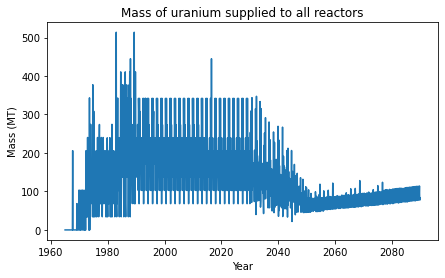
\includegraphics[scale=0.3]{figures/fuelsupply_scenarios_5.png}
        \caption{Total mass of uranium sent to all reactors at each time step.}
        \label{fig:totalfuel_5}
    \end{subfigure}
    \begin{subfigure}{0.4\textwidth}
        \centering
        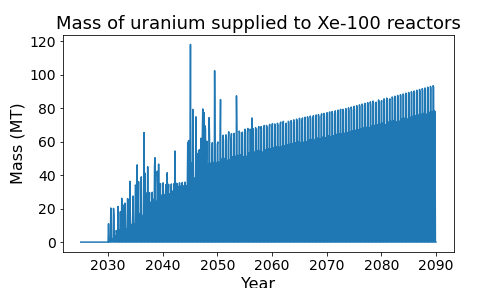
\includegraphics[scale=0.3]{figures/advancedRX_fuelsupply_scenarios_5.png}
        \caption{Total mass of uranium sent to Xe-100s at each time step.}
        \label{fig:haleu_5}
    \end{subfigure}
    \caption{Uranium mass sent to reactors in Scenario 5.}
    \label{fig:fuel_5}
\end{figure}


\begin{figure}
    \centering
    \begin{subfigure}{0.4\textwidth}
        \centering
        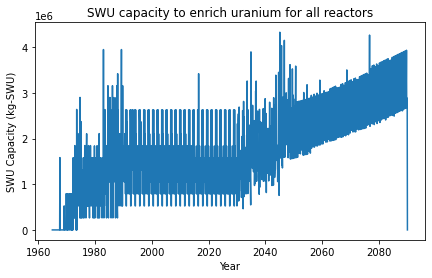
\includegraphics[scale=0.3]{figures/totalswu_scenarios_5.png}
        \caption{Total \gls{SWU} required to enrich uranium sent to all reactors at each time step.}
        \label{fig:totalswu_5}
    \end{subfigure}
    \begin{subfigure}{0.4\textwidth}
        \centering
        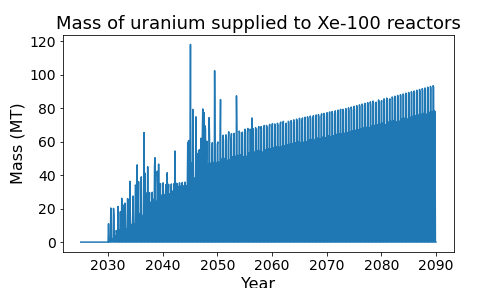
\includegraphics[scale=0.3]{figures/advancedRX_fuelsupply_scenarios_5.png}
        \caption{\gls{SWU} required to enrich uranium sent to Xe-100s at each time step.}
        \label{fig:haleuswu_5}
    \end{subfigure}
    \caption{\gls{SWU} required to enrich natural uranium in Scenario 5.}
    \label{fig:swu_5}
\end{figure}
